\newpage

\begin{center}
	\section{An\'alisis de resultados y conclusiones}
\end{center}

\noindent
\justify

De las iteraciones desarrolladas, la configuraci\'on de aletas que mejor desempe\~no obtuvo fue la tercera (10 aletas de $h=40 [mm]$, $\theta = 30 [\degree ]$ y bolas de: $7[cm]$, $5[cm]$ y $2.5[cm]$; como se observa en la Figura \ref{sol}), debido a que obtuvo la mayor energ\'ia cin\'etica media y la distribuci\'on de energ\'ia de impacto m\'as equitativa durante la etapa de molienda. Como se observa en la Figura \ref{resul4}, este sistema cumple el objetivo requerido por la planta de extracci\'on debido a que las esferas de $7 [cm]$ y $5 [cm]$ presentan la energ\'ia suficiente para disminuir el tama\~no de part\'icula de tallos y ramas, mientras que las bolas de $2.5 [cm]$ lograr\'an pulverizar el material por debajo de los $250 [\mu m]$.

\begin{figure}[h!]
\centering
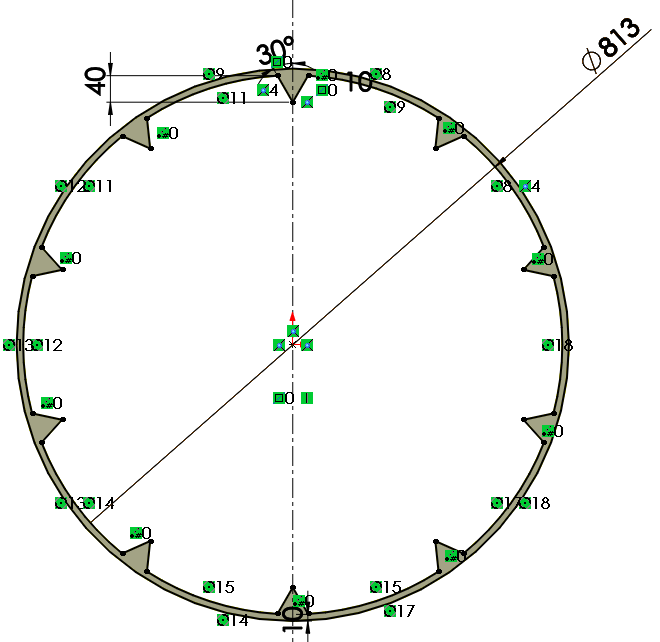
\includegraphics[width=\textwidth]{Images/Resultados/res.PNG}
\caption{Dise\~no funcional del molino.}
\label{sol}
\end{figure}